\section{Weiterentwicklung MobSF}
\label{Weiterentwicklung MobSF}
Ein Kernelement dieser Arbeit ist die Weiterentwicklung des Mobile Security Frameworks \textit{MobSF}. Die Funktionen des Frameworks sind bereits unter TODO aufgezeigt. Im Folgenden sind die Änderungen dargestellt, welche an dem Framework vorgenommen und veröffentlicht wurden.

\subsection{Allgemeine Verbesserungen}
Neben Verbesserungen, welche einem genauen Bereich (\textit{Windows-Phone}, \textit{iOS}, \textit{Android}) zuzuordnen sind, gibt es auch einige allgemeine Erweiterungen am \textit{Mobile Security Framework}. Diese sind im Folgenden dargestellt.

\subsubsection{Struktur}
Die Struktur von MobSF war bisher relativ flach. Auf der ersten Ebene findet man die Übergeordneten Module wie den \textit{ApiTester}, \textit{StaticAnalyzer}, \textit{DynamicAnalyzer} sowie den \textit{statischen Content}, \textit{Templates} und Kern-Module des \textit{MobSF}. Dies ist in der Abbildung \ref{fig:MobSFStrukOrig} verdeutlicht. Jedoch hatte die Struktur in den Modulen oft keine saubere Trennung der Aufgaben. So waren im \textit{StaticAnalyzer}-Modul sowohl \textit{iOS} wie auch \textit{Android}-Analyse in der \textit{views.py} zusammengefasst. Um hier eine klarere Trennung zu schaffen, wurde die \textit{views.py} aufgegliedert in drei Dateien:
\begin{description}
	\item[shared\_func.py: ] Die \textit{shared\_func.py} enthält alle Funktionen, welche sowohl für \textit{iOS} als auch \textit{Android} gebraucht werden. Beispiele sind die Erstellung von Hashes, das Generieren von PDFs oder das Entpacken von Archiven.
	
	\item[ios.py: ] Die Datei \textit{ios.py} enthält alle \textit{iOS} spezifischen Funktionen zur statischen Analyse.
	
	\item[android.py: ] Die Datei \textit{android.py} enthält alle \textit{Android} spezifischen Funktionen zur statischen Analyse.
	
	\item[windows.py: ] Die Datei \textit{windows.py} enthält alle \textit{Windows-Phone} spezifischen Funktionen zur statischen Analyse. Sie wurde nachträglich hinzugefügt (siehe \ref{Windows-Apps}), weshalb die Funktionen in der altern Struktur nicht auftauchen.
\end{description}
Dies ist im Detail in der Abbildung \ref{fig:MobSFStaticStrucVergl} dargestellt.

\begin{figure}
\dirtree{%
.1 Mobile-Security-Framework-MobSF/.
    .2 .git/.
    .2 APITester/.
    .2 downloads/.
    .2 DynamicAnalyzer/.
    .2 LICENSES/.
    .2 logs/.
    .2 MalwareAnalyzer/.
    .2 MobSF/.
    .2 static/.
    .2 StaticAnalyzer/.
    .2 templates/.
    .2 uploads/.
}
\label{fig:MobSFStrukOrig}
\caption{Strutkur MobSF auf der ersten Ebene}
\end{figure}

\begin{figure}
\centering
\begin{subfigure}{.5\textwidth}
  \dirtree{%
.1 StaticAnalyzer/.
    .2 [...].
    .2 views.py.
    	.3 key.
    	.3 PDF.
    	.3 Java.
    	.3 Smali.
    	.3 Find.
    	.3 ViewSource.
    	.3 ManifestView.
    	.3 StaticAnalyzer.
    	.3 GetHardcodedCertKeystore.
    	.3 ReadManifest.
    	.3 GetManifest.
    	.3 ValidAndroidZip.
    	.3 HashGen.
    	.3 FileSize.
    	.3 GenDownloads.
    	.3 zipdir.
    	.3 Unzip.
    	.3 FormatPermissions.
    	.3 CertInfo.
    	.3 WinFixJava.
    	.3 WinFixPython3.
    	.3 Dex2Jar.
    	.3 Dex2Smali.
    	.3 Jar2Java.
    	.3 Strings.
    	.3 ManifestData.
    	.3 ManifestAnalysis.
    	.3 CodeAnalysis.
    	.3 StaticAnalyzer\_iOS.
    	.3 ViewFile.
    	.3 readBinXML.
    	.3 HandleSqlite.
    	.3 iOS\_ListFiles.
    	.3 BinaryAnalysis.
    	.3 iOS\_Source\_Analysis.
}
  \caption{Alte Struktur}
  \label{fig:sub1}
\end{subfigure}%
\begin{subfigure}{.5\textwidth}
  \dirtree{%
.1 Mobile-Security-Framework-MobSF/.
    .2 [...].
    .2 views/.
		.3 android.py.
	    	.4 [...].
	    	.4 GetHardcodedCertKeystore.
	    	.4 ReadManifest.
	    	.4 GetManifest.
	    	.4 ValidAndroidZip.
	    	.4 Dex2Jar.
	    	.4 Dex2Smali.
	    	.4 Jar2Java.
	    	.4 [...].
		.3 ios.py.
	    	.4 StaticAnalyzer\_iOS.
	    	.4 ViewFile.
	    	.4 readBinXML.
	    	.4 HandleSqlite.
	    	.4 iOS\_ListFiles.
	    	.4 BinaryAnalysis.
	    	.4 iOS\_Source\_Analysis.
	    .3 windows.py.
	    	.4 [...].
	    	.4 \_\_binskim.
	    	.4 \_\_binscope.
	    	.4 [...].
		.3 shared\_func.py.
	    	.4 key.
	    	.4 FileSize.
	    	.4 HashGen.
	    	.4 Unzip.
	    	.4 PDF.
}
  \caption{Neue Struktur}
  \label{fig:sub2}
\end{subfigure}
\caption{Vergleich der Struktur von \textit{StaticAnalyzer}}
\label{fig:MobSFStaticStrucVergl}
\end{figure}

Im weiteren Verlauf der Weiterentwicklung und mit der Einführung von Code-Standards (siehe \ref{pylintering}) wurde die Struktur weiter verfeinert.

TODO

\subsubsection{Namedtuple vs. DICT}
TODO

\subsubsection{Code-Standards}
\label{pylintering}
Bei der Neu- oder Reimplementierung wurde auf die Verwendung von offiziellen Style-Guides geachtet. Insbesondere wurde der\textit{ PEP 8} Standard \footnote{\url{https://www.python.org/dev/peps/pep-0008/}} für Python verwendet, welcher die Lesbarkeit und Wartbarkeit von Python-Code verbessern soll. Um die Einhaltung des Standards zu gewährleisten, wurde das Tool \textit{Pylint} verwendet. Dieses prüft einen gegebenen Quellcode gegen den Code-Standard \textit{PEP 8} und kreiert entsprechende Warnungen für Abweichungen. Ursprünglich musste \textit{Pyling} auf der Konsole extra ausgeführt werden, jedoch können moderne Entwicklungsumgebungen wie \textit{Atom} \textit{Pylint} direkt einbinden und nutzen. Dies hat den Vorteil, dass bereits während dem Programmieren Verstöße gegen Standard oder Fehler wie zum Beispiel falsche Variablennamen entdeckt werden.\\

Für \textit{MobSF} wurde nicht von Anfang an mit Code-Standards entwickelt, weshalb zum Beispiel die Datei \textit{android.py} über 2000 Code-Zeilen mit über 1600 \textit{Pylint}-Fehler aufwies. Durch aufwendige Refaktorierungs- und Umstrukturierungsarbeiten konnte die Anzahl der Abweichungen massiv reduziert werden.\\

Daraus ergibt sich erhöhte Wartbarkeit sowie eine einfachere Entwicklung aufgrund weniger Merge-Konflikte. Dies ist möglich, da die jeweiligen Methoden je nach Funktionalität in entsprechende Module ausgelagert wurden und somit nur die eine, für die Funktion benötigte Datei, verändert und wieder in das Haupt-Projekt eingegliedert werden muss. Zuvor musste bei paralleler Entwicklung am Projekt auch nur eine kleine Änderung in die übergreifende Datei mit Änderungen einer parallel arbeitenden Partei zusammengeführt werden, was oftmals viel Arbeit bedeutet.

TODO pep8 vs flake8 vs xxx..

\subsubsection{strings}\label{ref:strings}
Zuerst wurde das MobSF um die Fähigkeit erweitert, eine iOS-Applikation mit dem \textit{strings}-Programm zu untersuchen. \textit{strings} durchsucht, insofern keine zusätzlichen Parameter übergeben werden, eine binäre Datei mach 4 aufeinander folgende ASCII-Elemente.\\

Dies hilft oft bei einer ersten Einschätzung der Anwendung, da oft eine grundlegende Funktionsweise und der Zweck der Software abgeleitet werden kann. Ebenso können eventuell unbeabsichtigt im Programm vergesse Strings in einer App aufgedeckt werden. Auch sind gelegentlich Funktionsnamen oder Kernel-Calls als String in einem Binary enthalten, was unter TODO zum Entdecken von verwundbaren Funktionen genutzt wird.\\

Sowohl \textit{Mac-OSX} wie auch \textit{Linux} haben ein integriertes \textit{string}-Kommando, welches jedoch \textit{Windows} fehlt. Um die Multi-Platform-Fähigkeit weiterhin zu gewährleisten, wurde die Funktionsweise in Python-Code abgebildet. Als Vorlage wurde ein bestehender Code von \textit{Stackoverflow} \footnote{\url{http://stackoverflow.com/a/17197027}} genutzt. Dieser lieferte jedoch eine wesentlich höhere Anzahl von Ergebnissen, da bestimmte Whitespace-Character ebenfalls beachtet wurden:
\begin{lstlisting}
> wc -l strings_test_*
	  85149 strings_test_orig
  	541393 strings_test_pyth
    626542 total
\end{lstlisting}

Da viele der zusätzlich aufgedeckten Strings jedoch nicht bei der Analyse geholfen, sonder eher das Auffinden relevanter Strings erschwert haben, wurde der Originalcode wie folgt angepasst:
\begin{lstlisting}
<<<<<<< Vor Anpassung
import string
=======
>>>>>>> Nach Anpassung

def strings(filename, min=4):
    """Print out all connected series of readable chars longer than min."""
    with open(filename, "rb") as f:
        result = ""
        for c in f.read():
<<<<<<< Vor Anpassung
            if c in string.printable:
=======
            if c in (
                    '0123456789'
                    'abcdefghijklmnopqrstuvwxyz'
                    'ABCDEFGHIJKLMNOPQRSTUVWXYZ'
                    '!"#$%&\'()*+,-./:;<=>?@[\\]^_`{|}~ '
            ):
>>>>>>> Nach Anpassung
                result += c
                continue
            if len(result) >= min and result[0].isalnum():
                yield "'" + result + "'"
            result = ""
\end{lstlisting}
Durch die Reduzierung der ausschlaggebenden Zeichen konnten die Ergebnisse optimiert werden, sodass eine effiziente Suche über Strings wieder möglich ist.

\subsubsection{PDF-Generation}
Um eine effiziente Weitergabe der Ergebnisse zu ermöglichen, besitzt das \textit{Mobile Security Framework} eine PDF-Export-Funktion. Die Implementierung ist dabei relativ einfach. Es wird eine neue HTML-Sicht geschaffen, welche anschließend über das das Python-Modul \textit{xhtml2pdf.pisa} als PDF geöffnet wird.

Eine solche Sicht wurde jeweils für alle Erweiterungen implementiert, welche in dieser Arbeit vorgenommen wurden.

\subsubsection{RPC-Service}\label{ref:XMLRPC}
Um eine Kommunikation zwischen verschiedenen Virtuellen Maschinen zu ermöglichen, wurde ein minimaler \textit{RPC-Server} in Python 3.5 entwickelt. Hierzu wurden verschiedene Ansätze untersucht. Getestet wurden hierzu die Python-Module \textit{Flask}, \textit{Requests}, \textit{xmlrpc} sowie \textit{RSA} zum Hinzufügen einer Authentisierung.

\paragraph{Flask}\label{ref:flask}
Flask ist ein schneller, minimaler Webserver. Mit nur sehr wenig Code es möglich, eine Schnittstelle bereit zu stellen. Ein Code mit zwei akzeptierenden Funktionen, basierend auf der Schnellstart-Anleitung\footnote{\url{http://flask.pocoo.org/docs/0.10/quickstart/}}, ist in Abbildung \ref{ref:rpc_client.py} dargestellt.
\begin{figure}
\begin{lstlisting}
from flask import Flask
app = Flask(__name__)

@app.route('/')
def hello_world():
	print("Execute command!")
    return 'Hello World!'
    
@app.route('/second_command/')
def not_hello_world():
	print("Execute second command!")
    return 'Goodbye World!'

if __name__ == '__main__':
    app.run()
\end{lstlisting}
\label{ref:rpc_client.py}
\caption{rpc\_client.py}
\end{figure}

Es wird eine minimale Anwendung erstellt, welche auf dem Pfad "\url{/}" lokal das \textit{print}-Statement ausführt und den Text 'Hello World!' zurück gibt. 
Wir die Anwendung unter dem Pfad "\url{/second_command/}" angesprochen, wird ein anderes \textit{print}-Statement ausgeführt und ein anderer Wert zurück gegeben. Auf diese Weise können schnell API-Funktionen auf verschiedene Pfade gelegt und angesprochen werden.

\paragraph{Requests}
\textit{Requests} ist ein Python-Modul, welche einfache Anfragen (sogenannte \textit{Requests}) über HTTP(S) ermöglicht. So ist es über ein kurzes Code-Snippet, dargestellt in Abbildung \ref{ref:rpc_server.py}, möglich die unter \ref{ref:rpc_client.py} aufgezeigt Schnittstelle anzusprechen.

\begin{figure}
\begin{lstlisting}
import requests

r = requests.get('http://localhost:5000')
print(r.text)

r = requests.get('http://localhost:5000/second_command/')
print(r.text)
\end{lstlisting}
\label{ref:rpc_server.py}
\caption{rpc\_server.py}
\end{figure}

Wird zuerst der Code \ref{ref:rpc_client.py} und anschließend der Code \ref{ref:rpc_server.py} ausgeführt, wird auf Server-Seite folgende Ausgabe erzeugt:
\begin{lstlisting}
 $ python3 rpc_server.py
Hello World!
Goodbye World!
\end{lstlisting}
Auf der Client-Seite erfolgt folgende Ausgabe:
\begin{lstlisting}
 $ python3 rpc_client.py
 * Running on http://127.0.0.1:5000/
Execute command!
127.0.0.1 - - [18/May/2016 19:10:56] "GET / HTTP/1.1" 200 -
Execute second command!
127.0.0.1 - - [18/May/2016 19:10:56] "GET /second_command/ HTTP/1.1" 200 -
\end{lstlisting}

Aufgrund dieser Basis wurde die erste Version des RPC-Servers implementiert.

\paragraph{xmlrpc mit rsa}
Bei der Eingliederung der Verbindung zwischen der virtuellem Maschine und dem Host wurde jedoch die Anforderung nach einer Möglichkeit zur Authentifizierung gefordert.\\

Zur Implementierung dieser Anforderung wurde das Python-Modul \textit{rsa} verwendet, welches sowohl für Python 2 wie auch Python 3 existiert. Die Funktionsweise ist dabei wie folgt.

TODO Zustandsdiagramm

Durch das Signieren einer bei jedem Funktionsaufruf neu generierten Challenge ist sichergestellt, dass nur der echte Host die Funktion aufruft und ist ebenfalls gegen Replay-Attacken geschützt TODO zu Replay.\\

Jedoch gab es bei der Implementierung über Flask sowie mit den verschiedenen Python-Versionen zwischen Server und Client verschiedene Probleme. So gibt es in Python 2 einen dedizierten Variablen-Typ namens \textit{string}, wohingegen Python 3 Strings in codierten Byte-Objekten speichert. Eine Konvertierung ist an sich möglich und wurde später auch umgesetzt. Jedoch legt \textit{Flask} eine weitere Ebene des Encodings über den übertragenen Inhalt, weshalb es leider nicht möglich war, die kryptographische Signatur fehlerfrei zu übertragen. Aus diesem Grund wurde nach weiteren und eventuell besser geeigneten Alternativen gesucht.\\

Nach einer kurzen Suche bot sich das Modul \textit{xmlrpclib} (Python 2)/\textit{xmlrpc} (Python 3) an. Es ermöglicht die Kommunikation über das standardisierte TODO XML-RPC-Protokoll und ist somit unabhängig von der Python-Version. Zudem können Daten transparent zwischen Server und Client übergeben werden.

\newpage
Es folgt ein kurzes Beispiel, in welcher ein Client eine \textit{hello\_world}-Funktion am Server aufruft.\\

Server-Code:
\begin{lstlisting}
from xmlrpc.server import SimpleXMLRPCServer

def hello_world(name):
	"""Return an Hello-World for a name"""
    return "Hello World {}!".format(name)

if __name__ == '__main__':
	# Open the Server on port 8000
    server = SimpleXMLRPCServer(("0.0.0.0", 8000))
    server.register_function(hello_world, "hello_world")
\end{lstlisting}
$ $\\
Client-Code (\textit{TARGET\_IP} sollte mit der richtigen IP-Adresse ersetzt werden):
\begin{lstlisting}
import xmlrpclib

proxy  = xmlrpclib.ServerProxy(
                "http://{}:{}".format(
                    TARGET_IP, 8000
                )
            )
print proxy.hello_world("John Doe")
\end{lstlisting}
$ $\\
Output des Clients:
\begin{lstlisting}
Hello World John Doe!
\end{lstlisting}

Durch den minimalen eingriff von \textit{xmlrpc} in die Kommunikation, konnte die kryptographische Signatur als \textit{base64} codiertes Datum übergeben werden. Im Folgenden sind kurz die Kern-Funktionen des RSA-Checks aufgezeigt.\\

Client-Code:
\begin{lstlisting}
def _get_token():
    """Get the authentication token for windows vm xmlrpc client."""
    challenge = proxy.get_challenge()
    priv_key = rsa.PrivateKey.load_pkcs1(
        open(settings.WINDOWS_VM_SECRET).read()
    )
    signature = rsa.sign(challenge, priv_key, 'SHA-512')
    sig_b64 = base64.b64encode(signature)
    return sig_b64
    
print proxy.test_challenge(_get_token())
\end{lstlisting}
\newpage
Server-Code:
\begin{lstlisting}
def _check_challenge(signature):
    signature = base64.b64decode(signature)
    try:
        rsa.verify(challenge.encode('utf-8'), signature, pub_key)
        print("[*] Challenge successfully verified.")
        _revoke_challenge()
    except rsa.pkcs1.VerificationError:
        print("[!] Received wrong signature for challenge.")
        raise Exception("Access Denied.")
    except (TypeError, AttributeError):
        print("[!] Challenge already unset.")
        raise Exception("Access Denied.")

def get_challenge():
    """Return an ascii challenge to validate authentication in _check_challenge."""
    global challenge
    # Not using os.urandom for Python 2/3 transfer errors
    challenge = ''.join(
        random.SystemRandom().choice(string.ascii_uppercase + string.digits) for _ in range(256)
    )
    return "{}".format(challenge)
    
def test_challenge(signature):
    """Test function to check if rsa is working."""
    _check_challenge(signature)
    print("Check complete")
    return "OK!"
\end{lstlisting}
Durch diese Art der Implementierung ist eine sichere, zuverlässige, effiziente und leicht erweiterbare Kommunikation zwischen Host und virtueller Maschine möglich.


\subsection{Windows-Apps}
\label{Windows-Apps}
Auch wenn die Zukunft der Handy-Sparte von Windows derzeit oftmals in Diskussion steht, geht der Trend zur Entwicklung auf gerade sein Windows 8 und der damit eingeführten TODO Window Unified Platform hin zur Entwicklung von Apps. Der Vorteil, dass diese Apps sowohl auf Windows auf einem PC wie auch auf Handy lauffähig sind, ist schwer bestreiten, macht jedoch eine Umfassende Prüfung der Sicherheit umso wichtiger.\\

Bisher hat das \textit{Mobile Security Framework} noch keine Möglichkeit zur Prüfung von Windows-Apps bereitgestellt. Im Folgenden sind die im Rahmen dieser Arbeit implementierten Features beschrieben.

\subsubsection{Windows Phone Formats}
Um eine App analysieren zu können, muss zu aller erst das File-Format betrachtet und verarbeitet werden. Leider sind im Windows-Umfeld diverse Formate gängig, von welchen im Folgenden einige in Hinblick auf Aufbau und Schutz analysiert werden.

\paragraph{xap}
\textit{XAP} ist ein Format für Windows-Phone-Apps ab \textit{Windows Phone 7} und enthält oft Silverlight-Applikationen.

Ursprünglich war ein \textit{XAP}-File einfach ein ein \textit{ZIP}-Archiv, mit allen Dateien der App. Aus einem solchen \textit{XAP}-File konnte der Inhalt über folgende Schritte einfach gewonnen werden:
\begin{enumerate}
	\item \textit{XAP}-File herunterladen
	\item evtl. Dateiendung von "`.xap"' auf "`.zip"' ändern
	\item mit einem gängigen Archiv-Programm (z.B. 7-Zip) entpacken
\end{enumerate}
Anschließend liegen allen Dateien der App im Extraktions-Ordner.\\

Leider sind \textit{XAP}-Files häufig durch sogenanntes \textit{DRM} (\textit{Digital Rights Management}) geschützt. So lässt sich bei vielen aktuellen XAP-Files folgender Header feststellen:
\begin{lstlisting}
<WRMHEADER xmlns="http://schemas.microsoft.com/DRM/2007/03/PlayReadyHeader" version="4.0.0.0">
	<DATA>
		<PROTECTINFO>
			<KEYLEN>16</KEYLEN>
			<ALGID>AESCTR</ALGID>
		</PROTECTINFO>
		<KID>5zhQkM1z5kq6HCCYD9nceQ==</KID>
		<LA_URL>http://microsoft.com/</LA_URL>
			<CUSTOMATTRIBUTES xmlns="">
				<S>rtXfkbbz4yuPNGrzjQc9yA==</S>
				<KGV>0</KGV>
			</CUSTOMATTRIBUTES>
		<CHECKSUM>TpkeZrwUjIY=</CHECKSUM>
	</DATA>
</WRMHEADER>
\end{lstlisting}

\url{http://forum.xda-developers.com/showpost.php?p=34246750&postcount=3}


The encrypted XAPs use AESCTR, PlayReady. First 32 bytes are a header, last two dwords are a length, the first half (BigEndian) is the 'payload' (actual app(+more?)) and the second half is always -8 bytes. Then comes the 'mal'-formed XML containign PlayReady definitions etc, including base64 encoded key ids etc. I'd like to see someone on custom rom P7 wireshark their network while using a MITM attack (SSL obviously) using an SSL cert accepted as root ca in the phone to see if we can dump any plaintext DRM keys per app, maybe a solid method can be made. For now, not sure. I've been working on it. Key lengths are 16 bytes. I can brute 12 bytes in one month but 16 would take a lot longer. You could also install a custom rom with wdmc on the phone and copy the entire folders off, restructured a little though, unpacked. Hope this helps someone else. All based on PlayReady DRM bs. Smooth Streaming in IIS can support PR too for instance (WRMHEADER aka PlayReady headers):
\url{http://forum.xda-developers.com/showthread.php?t=2046702}

VM + extraction-tool?

Mime-Type: application/x-silverlight-app

\paragraph{appx}
\textit{APPX} ersetzt ab Windows 8.1 das \textit{XAP}-Format.

Extraktion kann über das in Python integrierte Modul \textit{zipfile} erfolgen.
\begin{lstlisting}
import zipfile
files=[]
with zipfile.ZipFile(APP_PATH, "r") as z:
        z.extractall(EXT_PATH)
        files=z.namelist()
return files
\end{lstlisting}
Mime-Type:
\begin{lstlisting}
APPX_MIME = [
    'application/octet-stream',
    'application/vns.ms-appx',
    'application/x-zip-compressed'
]
\end{lstlisting}

\paragraph{appxbundle}

\begin{lstlisting}
['AugmentendApplicationAppx.appx', 'DumbSmash.WindowsPhone_1.1.0.15_language-it.appx', 'DumbSmash.WindowsPhone_1.1.0.15_scale-100.appx', 'DumbSmash.WindowsPhone_1.1.0.15_scale-120.appx', 'DumbSmash.WindowsPhone_1.1.0.15_scale-140.appx', 'AppxMetadata/AppxBundleManifest.xml', 'AppxBlockMap.xml', '[Content_Types].xml', 'AppxSignature.p7x']
\end{lstlisting}

MIME-Type
file --mime-type -b filename

\subsubsection{Virtuelle Maschine zur Analyse von Windows-Apps}
Die virtuelle Maschine zur Analyse von Windows Applikationen setzt sich aus TODO Komponenten zusammen. Für die Software-Komponenten wird ein Installer im Rahmen dieser Arbeit erstellt und zur Verfügung gestellt.\\

Als erstes muss ein Betriebssystem für die Analyse-VM gewählt werden. Normalerweise wäre Windows 7 aufgrund der geringeren Ressourcenauslastung die erste Wahl für Windows-Analyse-Maschinen. Da jedoch der Windows-Phone-Simulator erst ab Windows 8.1 64-Bit unterstützt wird, sollte in Hinsicht auf die dynamische Analyse davon abgesehen und Windows 8.1 64-Bit oder höher verwendet werden. Hier wurde Windows 10 64-Bit verwendet.\\

Eine weitere Voraussetzung ist Python 3. Getestet wurde in dieser Arbeit mit Python 3.5.2 32-Bit.\\

Für die restliche Installation wurde ein Installer angefertigt, der die restlichen notwendigen Programme herunterlädt und die Installationen anstößt. Das File ist im Anhang unter TODO zu finden. Genutzt wurden die Bibliotheken \textit{urllib}, \textit{configparser} und \textit{zipfile} sowie \textit{os} zur Ausführung.\\

Heruntergeladen und Installiert werden folgende Komponenten:
\begin{itemize}
	\item binskim
	\item binscope
\end{itemize}

Diese werden im Abschnitt \ref{ref:WeitMobEingTools} vorgestellt.\\

Die Ordnerstruktur wurde dabei anfangs wie folgt aufgebaut:
  \dirtree{%
.1 C:/.
    .2 [...].
    .2 MobSF/.
    	.3 Config/.
    		.4 config.txt.
    	.3 Download/.
    	.3 Tools/.    	
}

Um die Kompatibilität mit verschiedenen Systemkonfigurationen zu erhöhen, wurde später statt C die Ordner des Benutzers für die Speicherung der Programme verwendet.\\

Die \textit{config.txt} enthält Inhalte, welche zentral Abgelegt und für verschiedene Skripte eine wichtige Rolle spielen. Ein Beispiel wäre der Pfad zum Verzeichnis, in welchem die Tools gespeichert werden.\\

Der Downloads-Ordner hält die durch das Setup-Skript heruntergeladenen Binaries, der Tools-Ordner die installierten Tools.

\subsubsection{setup.py}
Die Datei \textit{setup.py} wird über zwei verschiedene Wege gerufen, je nach dem ob MobSF vollständig auf Windows installiert wird oder nur die statische Analyse auf dem Windows-System ausgeführt werden soll. Je nach Aufrufweise werden verschiedene Arbeitsschritte ausgeführt und auch verschiedene Python-Versionen verwendet, weshalb manche Funktionen sowohl Python 2 wie 3 kompatibel gestaltet sind.

\paragraph{MobSF auf Windows}
Wird MobSD vollständig auf Windows installiert, wird das Setup-Script einmalig aus der \textit{settings.py} aufgerufen. Dabei wird Python 2 verwendet. Anfangs wird das mit dem Download mitgelieferte Config-File in den richtigen Ordner des User-Kontext kopiert. Anschließend wird das Config-File über das ConfigParser-Modul geladen. Daraufhin werden alle notwendigen Ordner berechnet, in die Config geschrieben und angelegt. Damit sind die Vorbereitungen bezüglich der Config und der Ordner abgeschlossen.\\

Anschließend wird \textit{nuget} heruntergeladen. \textit{nuget} ist ein Paket-Manager für Windows, über welchen später \textit{BinSkim} installiert wird. Der Download ist in Python relativ einfach zu implementieren, wie in folgendem Code-Fragment dargestellt ist.
\begin{lstlisting}
# Open File
nuget_file_local = open(
	os.path.join(mobsf_subdir_tools, nuget_file_path), 
	"wb"
)

# Downloading File
print("[*] Downloading nuget..")
nuget_file = urlrequest.urlopen(nuget_url)

# Save content
print("[*] Saving to File {}".format(nuget_file_path))

# Write content to file
nuget_file_local.write(bytes(nuget_file.read()))

# Aaaand close
nuget_file_local.close()
\end{lstlisting}

Anschließend wird \textit{BinSkim} über \textit{nuget} installiert. Dazu wird \textit{nuget} mit verschiedenen Parametern aufgerufen.
\begin{lstlisting}
# Execute nuget to get binkim
output = subprocess.check_output(
    [
        nuget,
        "install", binskim_nuget, '-Pre',
        '-o', mobsf_subdir_tools
    ]
)
\end{lstlisting}
Anschließend wird wird aus den installierten Dateien die Binaries für \textit{BinSkim} \textit{x86} sowie \textit{x64} gesucht und in der Config-Datei gespeichert.\\

Als letztes Tool wird \textit{BinScope} installiert. Dies ist leider nicht über \textit{nuget} möglich. Daher muss eine MSI-Datei heruntergeladen und anschließend installiert werden. Dabei muss der Installationspfad entsprechend gesetzt werden. Der Quellcode kann dem Appendix unter TODO entnommen werden.\\

Um sicherzustellen, dass das Setup-Script nicht mehrmals ausgeführt wird, wird zuletzt ein Lock-File platziert. Bei erneutem Start der Anwendung wird auf dieses geprüft und falls es existiert eine erneute Installation übersprungen.

\paragraph{Statische Analyse auf Windows}
Wird nur die statische Analyse auf Windows durchgeführt, wird das Setup-Script direkt mit Python 3 ausgeführt. Dabei wird ähnlich zur Installation auf Windows zuerst das Config-File initialisiert und anschließend die Ordner erstellt. Auch werden \textit{nuget}, \textit{BinSkim} und \textit{BinScope} installiert.\\

Zusätzlich zur lokalen Installation wird jedoch ein XMLRPC-Server installiert und konfiguriert. Die genaue Funktionsweise dieses Services ist unter \ref{ref:XMLRPC} beschrieben.\\

Von Ajin Abraham, eines Contributors zu MobSF, wurde nach der Implementierung ein ergänzendes Video zur Installation erstellt und auf Youtube veröffentlicht\footnote{\url{https://www.youtube.com/watch?v=17ilENuMj58}}.

\subsubsection{Statische Analyse}
Um die drei marktführenden mobilen Betriebssysteme mit \textit{MobSF} abzudecken, wurden Funktionen für Windows-Phone-Apps hinzugefügt.

Zur statischen Analyse wurde das Tool \textit{binskim} von Microsoft getestet \footnote{\url{https://github.com/Microsoft/binskim/releases}}. Das Tool analysiert Compiler-Flags und verschiedenste andere statisch feststellbare Eigenschaften, bewertet diese und gibt die Ergebnisse im SARIF-Format\footnote{\url{https://github.com/sarif-standard/sarif-spec/}} zurück. Leider ist das Tool nur unter Windows ausführbar. Da \textit{MobSF} jedoch auch auf Linux und Mac OS X lauffähig sein soll, wird im folgenden eine virtuelle Windows-Maschine zur statischen und dynamischen Analyse verwendet.
\\\\
\_CRT\_SECURE\_NO\_WARNINGS

\paragraph{Files}
TODO

\paragraph{Bad Functions}
Ebenso wie bei iOS wurde auch hier eine Extraktion der Strings aus dem Binary implementiert. Genutzt wurde dafür die unter \ref{ref:strings} entwickelte Implementierung des Strings-Kommandos in Python.\\

In diesen Strings sind ebenfalls die Namen der verwendeten Funktionen vorhanden, sodass auch hier eine Suche nach bekannterweise verwundbaren Funktionen implementiert wurde.

\subsubsection{Eingebundene Tools}\label{ref:WeitMobEingTools}
Im Folgenden werden die für die Analyse von Windows-Apps eingebundenen Tools kurz vorgestellt.

TODO: https://blog.netspi.com/verifying-aslr-dep-and-safeseh-with-powershell/

\paragraph{Binskim}
nuget download
A binary static analysis tool that provides security and correctness results for Windows portable executables. 

This repository contains source code for BinSkim, a portable executable scanner that validates compiler/linker settings and other security-relevant binary characteristics.

TODO übersetzten
\begin{description}
	\item[LoadImageAboveFourGigabyteAddress] 64-bit images should have a preferred base address above the 4GB boundary to prevent triggering an Address Space Layout Randomization (ASLR) compatibility mode that decreases security.
	\item[DoNotIncorporateVulnerableDependencies] Binaries should not take dependencies on code with known security vulnerabilities.
	\item[DoNotShipVulnerableBinaries] Do not ship obsolete libraries for which there are known security vulnerabilities.
	\item[BuildWithSecureTools] Application code should be compiled with the most up-to-date tool sets possible to take advantage of the most current compile-time security features.
	\item[EnableCriticalCompilerWarnings] Binaries should be compiled with a warning level that enables all critical security-relevant checks.
	\item[EnableControlFlowGuard] Binaries should enable the compiler control guard feature (CFG) at build time to prevent attackers from redirecting execution to unexpected, unsafe locations.
	\item[EnableAddressSpaceLayoutRandomization] Binaries should linked as DYNAMICBASE to be eligible for relocation by Address Space Layout Randomization (ASLR).
	\item[DoNotMarkImportsSectionAsExecutable] PE sections should not be marked as both writable and executable.
	\item[EnableStackProtection] Binaries should be built with the stack protector buffer security feature (/GS) enabled to increase the difficulty of exploiting stack buffer overflow memory corruption vulnerabilities.
	\item[DoNotModifyStackProtectionCookie] Application code should not interfere with the stack protector.
	\item[InitializeStackProtection] Binaries should properly initialize the stack protector (/GS) in order to increase the difficulty of exploiting stack buffer overflow memory corruption vulnerabilities.
	\item[DoNotDisableStackProtectionForFunctions] Application code should not disable stack protection for individual functions.
	\item[EnableHighEntropyVirtualAddresses] Binaries should be marked as high entropy Address Space Layout Randomization (ASLR) compatible.
	\item[MarkImageAsNXCompatible] Binaries should be marked as NX compatible to help prevent execution of untrusted data as code.
	\item[EnableSafeSEH] X86 binaries should enable the SafeSEH mitigation to minimize exploitable memory corruption issues.
	\item[DoNotMarkWritableSectionsAsShared] Code or data sections should not be marked as both shared and writable.
	\item[DoNotMarkWritableSectionsAsExecutable] PE sections should not be marked as both writable and executable.
	\item[SignSecurely] Images should be correctly signed by trusted publishers using cryptographically secure signature algorithms.
\end{description}

Der originale Text sowie längere Beschreibungen sind dem Output des Kommandos
\begin{lstlisting}
BinSkim.exe exportRules output.json
\end{lstlisting}
zu entnehmen. Ebenfalls ist der Output angehängt unter TODO.

\paragraph{Binscope}
x64 vs x68
https://github.com/DominikSchlecht/Mobile-Security-Framework-MobSF/issues/10

Fehler-Beschreibungen
\begin{description}
	\item[ATLVersionCheck] Verifies that ATL headers used to build the binary are known good. For COM only.
	\item[ATLVulnCheck]  Detects classes implementing IPersistStreamInit that have potentially vulnerable property map entries. For COM only.
	\item[APTCACheck]  Reports a failure if the binary being verified is a managed assembly, has a strong name signature, and bears the APTCA attribute (AllowPartiallyTrustedCallersAttribute). Such assemblies can be potentially dangerous and should not be shipped without a thorough security review.
	\item[SectCheck] Reports a failure if the PE-format binary being verified has sections marked as shared and writable. Having such sections is a potential security vulnerability, and their use should be avoided.
	\item[GSCheck] Verifies that the /GS compiler flag was used to compile all components of the binary and shows detailed information per object in the binary. It is possible that only part of the object files in a binary were built with /GS. In this case you will need to find the owner of non-/GS-compiled objects or libraries and request a compliant version. Note: GSCheck needs access to the debug symbols for the binary. Ensure that the correct symbols are able to be located 
	(for example by setting $_NT_SYMBOL_PATH=SRV*\\symbols\\symbols$).
	\item[SafeSEHCheck]  Verifies that the image was linked using /SAFESEH. Not using /SAFESEH undermines the protection provided by /GS. Note - In order to link an image with /SAFESEH, all object files and lib files must be /SAFESEH-compatible.
	\item[FPCheck] Identifies images having global function pointers. Overriding static buffers can cause global function pointers to be overwritten, which may expose a security vulnerability. This is not covered by /GS protection; therefore, if you have global function pointers, you may want to examine use of static/global buffers in your code to make sure there are no possible security issues. This check is not enforced by SDL, but it is strongly recommended that you check use of your static buffers to make sure no buffer overruns are possible. FPCheck requires that symbols be present (see the /GS check note above).
	\item[SicCheck]  Identifies images that have non-/GS-friendly initialization. When using /GS, the executable needs some way to initialize the /GS infrastructure at load time, and usually it is done in CRT startup or similar functions. However, if the executable is linked in such a way that no standard code is executed at startup (such as with /NOENTRY linker option) and no custom /GS-startup routine is provided, that image will be left unprotected. This check identifies these images.
	\item[CompilerCheck] Identifies images that contain C or C++ modules compiled with a compiler older than the version required by the SDL. Specifically, BinScope checks that the C/C++ compiler (cl.exe) is at least version 14.00.50727 and the CVTRES compiler, the MASM compiler and the linker are at least version 8.00.50727. Those are the versions of the tools contained in Visual Studio 2005.
	\item[DBCheck] Checks if a binary has opted into the ASLR feature.
	\item[SNCheck] Checks for use of strong-named assemblies. A strong name is a digital signature representing a cryptographically unique name for a managed assembly. Integrity of information is protected by digital signature. No piece of the strong name and no bits in the assembly body can be modified without rebuilding the assembly.
  \item[NXCheck] Checks if a binary has opted into Hardware Data Execution Prevention.
\end{description}
\url{http://www.dotnetspark.com/kb/3784-binscope-binary-analyzer.aspx}

\paragraph{Decompiler?}
http://www.telerik.com/products/decompiler.aspx


\subsubsection{Dynamische Analyse von Windows-Apps}
Für das Remote-System sollte beachtet werden, dass für den Phone-Simulator von Microsoft Windows 8.1 Pro 64-Bit oder höher benötigt wird.

Verwendet wird ein \textit{Windows 10 64-Bit} mit \textit{Python 3.5} und \textit{Visual Studio 2015} Community Edition verwendet. Bis auf das Betriebssystem sind keine kostenpflichtigen Programme beteiligt.

windows driver kit für windbg

\subsection{iOS-Apps}
TODO

\subsubsection{Umwandeln app zu ipa}
Die Umwandlung von \textit{.app} zu \textit{.ipa} ist über wenige händische Schritte zu verwirklichen. Kompiliert man eine App in XCode, wird diese unter einem bestimmten Pfad abgelegt. Der Standardpfad unter XCode 8 ist \textit{/Users/dominik/Library/Developer/Xcode/DerivedData/}. Alternativ kann der Pfad den Projekt-Einstellung in XCode über \textit{File $\rightarrow$ Projects Settings} entnommen werden.\\

Die Struktur des \textit{DerivedData}-Ordner ist unter \ref{ref:deriveddata} dargestellt.
\begin{figure}
\dirtree{%
.1 DerivedData/.
    .2 \textit{Appname}-\textit{random}/.
    .2 \textit{Appname2}-\textit{random}/.
    	.3 Build/.
    		.4 Products/.
    			.5 \textit{Platform}/.
    				.6 \textit{Appname}.app.
    	.3 Index/.
    	.3 Logs/.
    	.3 TextIndex/.
    	.3 info.plist.
    	.3 scm.plist.    	
}
\label{ref:deriveddata}
\caption{Struktur des DerivedData-Ordners}
\end{figure}

Die \textit{.app}-Datei kann nun per Drag-n-Drop in den App-Bildschirm von \textit{ITunes} gezogen werden. Anschließend wird die App in ITunes angelegt (siehe Grafik \ref{fig:itunes_app}). Wird die App per Drag-n-Drop wieder aus \textit{ITunes} in den Finder gezogen, wird die App als IPA-File abgelegt.

\begin{figure}[htbp]
	\centering
	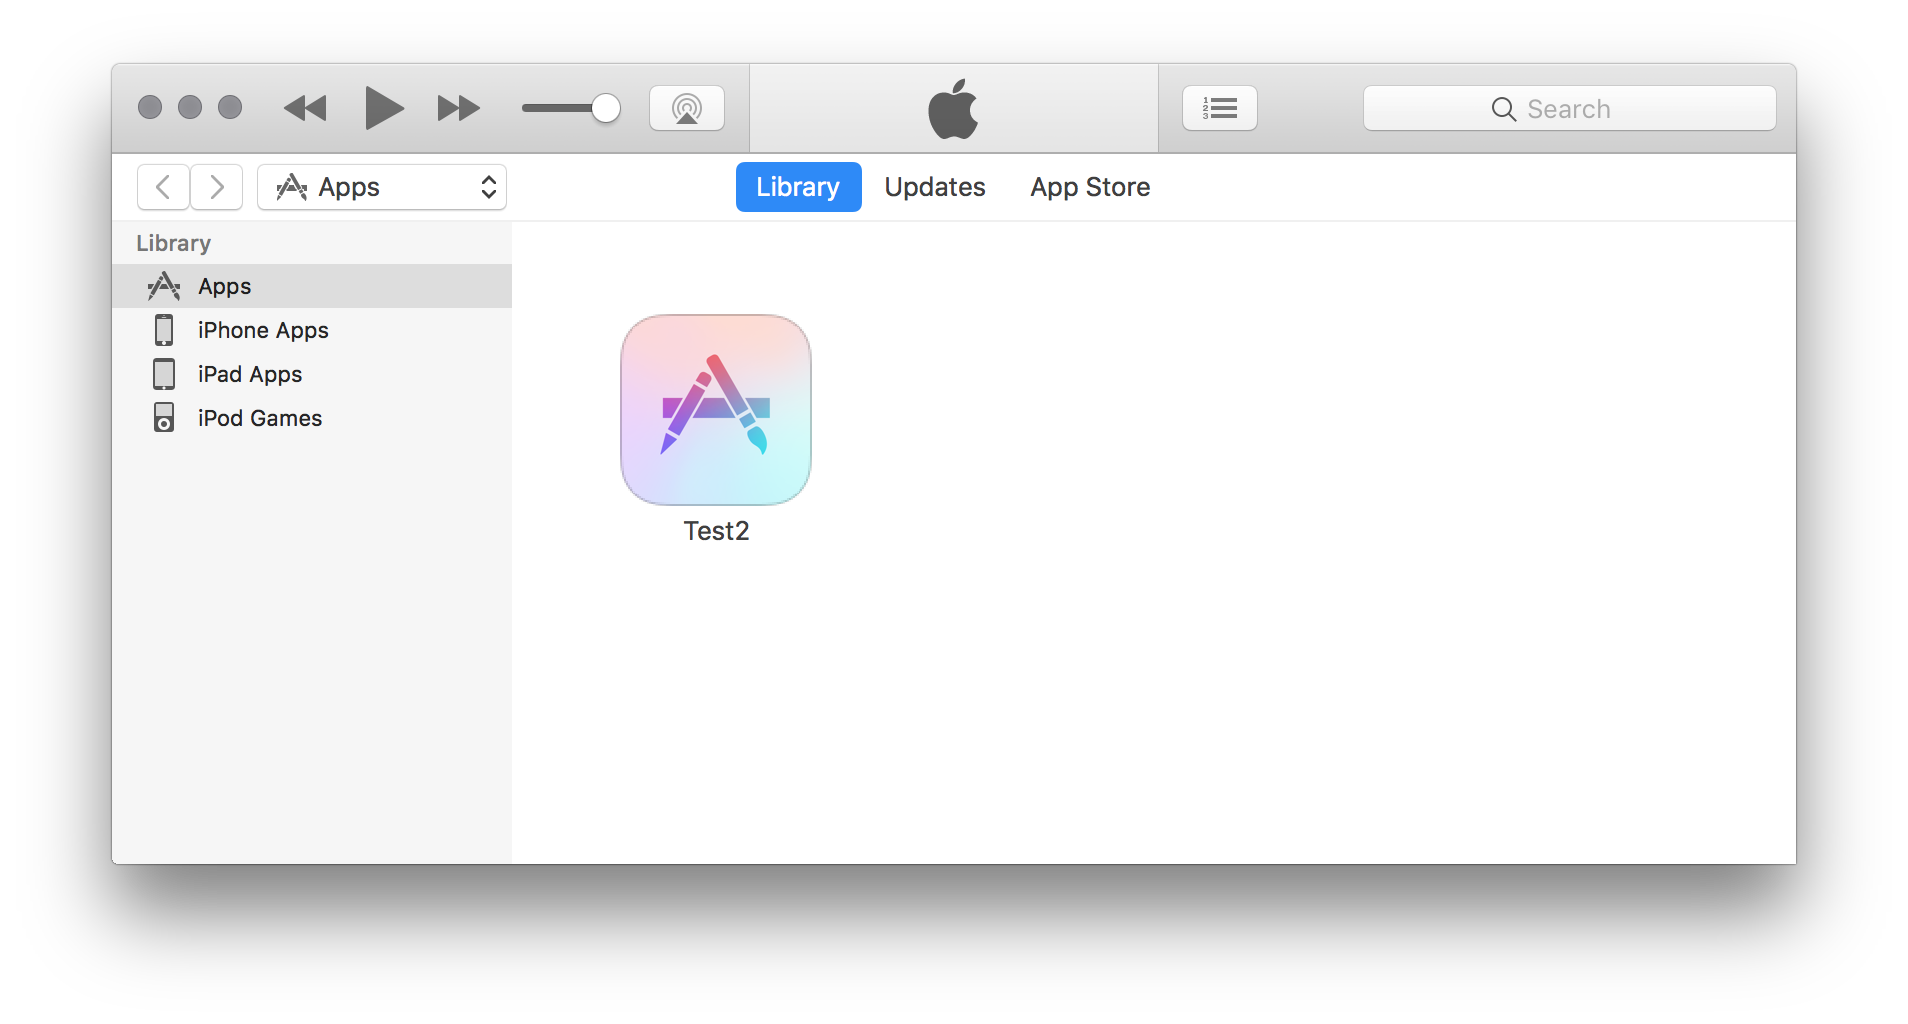
\includegraphics[width=\textwidth]{bilder/pentest_mobile_anwendungen/weiterentw_mobsf/itunes_app.png}
	\caption{ITunes-App-Fenster}
	\label{fig:itunes_app}
\end{figure}

\subsubsection{iOS-Permissions}
In den aktuellen Version von iOS müssen Berechtigungen, welche die App zur Laufzeit anfordert, in der \textit{info.plist} angekündigt werden. Im Folgenden sind die derzeit möglichen Berechtigungen aufgeführt.

\begin{description}
	\item[NSAppleMusicUsageDescription]  Specifies the reason for your app to use the media library. See NSAppleMusicUsageDescription for details.
	\item[NSBluetoothPeripheralUsageDescription] Specifies the reason for your app to use Bluetooth. See NSBluetoothPeripheralUsageDescription for details.
	\item[NSCalendarsUsageDescription] Specifies the reason for your app to access the user’s calendars. See NSCalendarsUsageDescription for details.
	\item[NSCameraUsageDescription] Specifies the reason for your app to access the device’s camera. See NSCameraUsageDescription for details.
	\item[NSContactsUsageDescription] Specifies the reason for your app to access the user’s contacts. See NSContactsUsageDescription for details.
	\item[NSHealthShareUsageDescription] Specifies the reason for your app to read the user’s health data. See NSHealthShareUsageDescription for details.
	\item[NSHealthUpdateUsageDescription] Specifies the reason for your app to make changes to the user’s health data. See NSHealthUpdateUsageDescription for details.
	\item[NSHomeKitUsageDescription] Specifies the reason for your app to access the user’s HomeKit configuration data. See NSHomeKitUsageDescription for details.
	\item[NSLocationAlwaysUsageDescription] Specifies the reason for your app to access the user’s location information at all times. See NSLocationAlwaysUsageDescription for details.
	\item[NSLocationUsageDescription] Unused. Use NSLocationWhenInUseUsageDescription or NSLocationAlwaysUsageDescription instead. See NSLocationUsageDescription for details.
	\item[NSLocationWhenInUseUsageDescription] Specifies the reason for your app to access the user’s location information while your app is in use. See NSLocationWhenInUseUsageDescription for details.
	\item[NSMicrophoneUsageDescription] Specifies the reason for your app to access any of the device’s microphones. See NSMicrophoneUsageDescription for details.
	\item[NSMotionUsageDescription] Specifies the reason for your app to access the device’s accelerometer. See NSMotionUsageDescription for details.
	\item[NSPhotoLibraryUsageDescription] Specifies the reason for your app to access the user’s photo library. See NSPhotoLibraryUsageDescription for details.
	\item[NSRemindersUsageDescription] Specifies the reason for your app to access the user’s reminders. See NSRemindersUsageDescription for details.
	\item[NSVideoSubscriberAccountUsageDescription] Specifies the reason for your app to access the user’s TV provider account. See NSVideoSubscriberAccountUsageDescription for details.
\end{description}

\url{https://developer.apple.com/library/content/documentation/General/Reference/InfoPlistKeyReference/Articles/CocoaKeys.html#//apple_ref/doc/uid/TP40009251-SW47}

Um in \textit{MobSF} die Berechtigungen auszulesen, wurde dementsprechend die \textit{info.plist} ausgelesen und auf die entsprechenden Einträge geprüft. Da die Datei jedoch im Binärformat vorliegt, muss diese zuerst umgewandelt werden. Dies kann über das in XCode enthaltene Tool \textit{plutil} erreicht werden. Der Aufruf ist dabei wie folgt:
\begin{lstlisting}
plutil -convert xml1 info.plist
\end{lstlisting}
Anschließend kann über das in Python enthaltene Modul \textit{plistlib} wie folgt auf die Einträge zugegriffen werden:
\begin{lstlisting}
p_list = plistlib.readPlistFromString(read_bin_xml(converted_info_plist_file))
if "NSBluetoothPeripheralUsageDescription" in p_list:
        print("Bluetooth-Permission found!")
\end{lstlisting}

in MobSF wird auf diese Art und Weise die \textit{info.plist}-Datei verarbeitet und die Ergebnisse in der Web-Oberfläche dargestellt. Das Ergebnis für eine App mit Bluetooth-Berechtigung ist in Grafik \ref{fig:permission_check} dargestellt.

\begin{figure}[htbp]
	\centering
	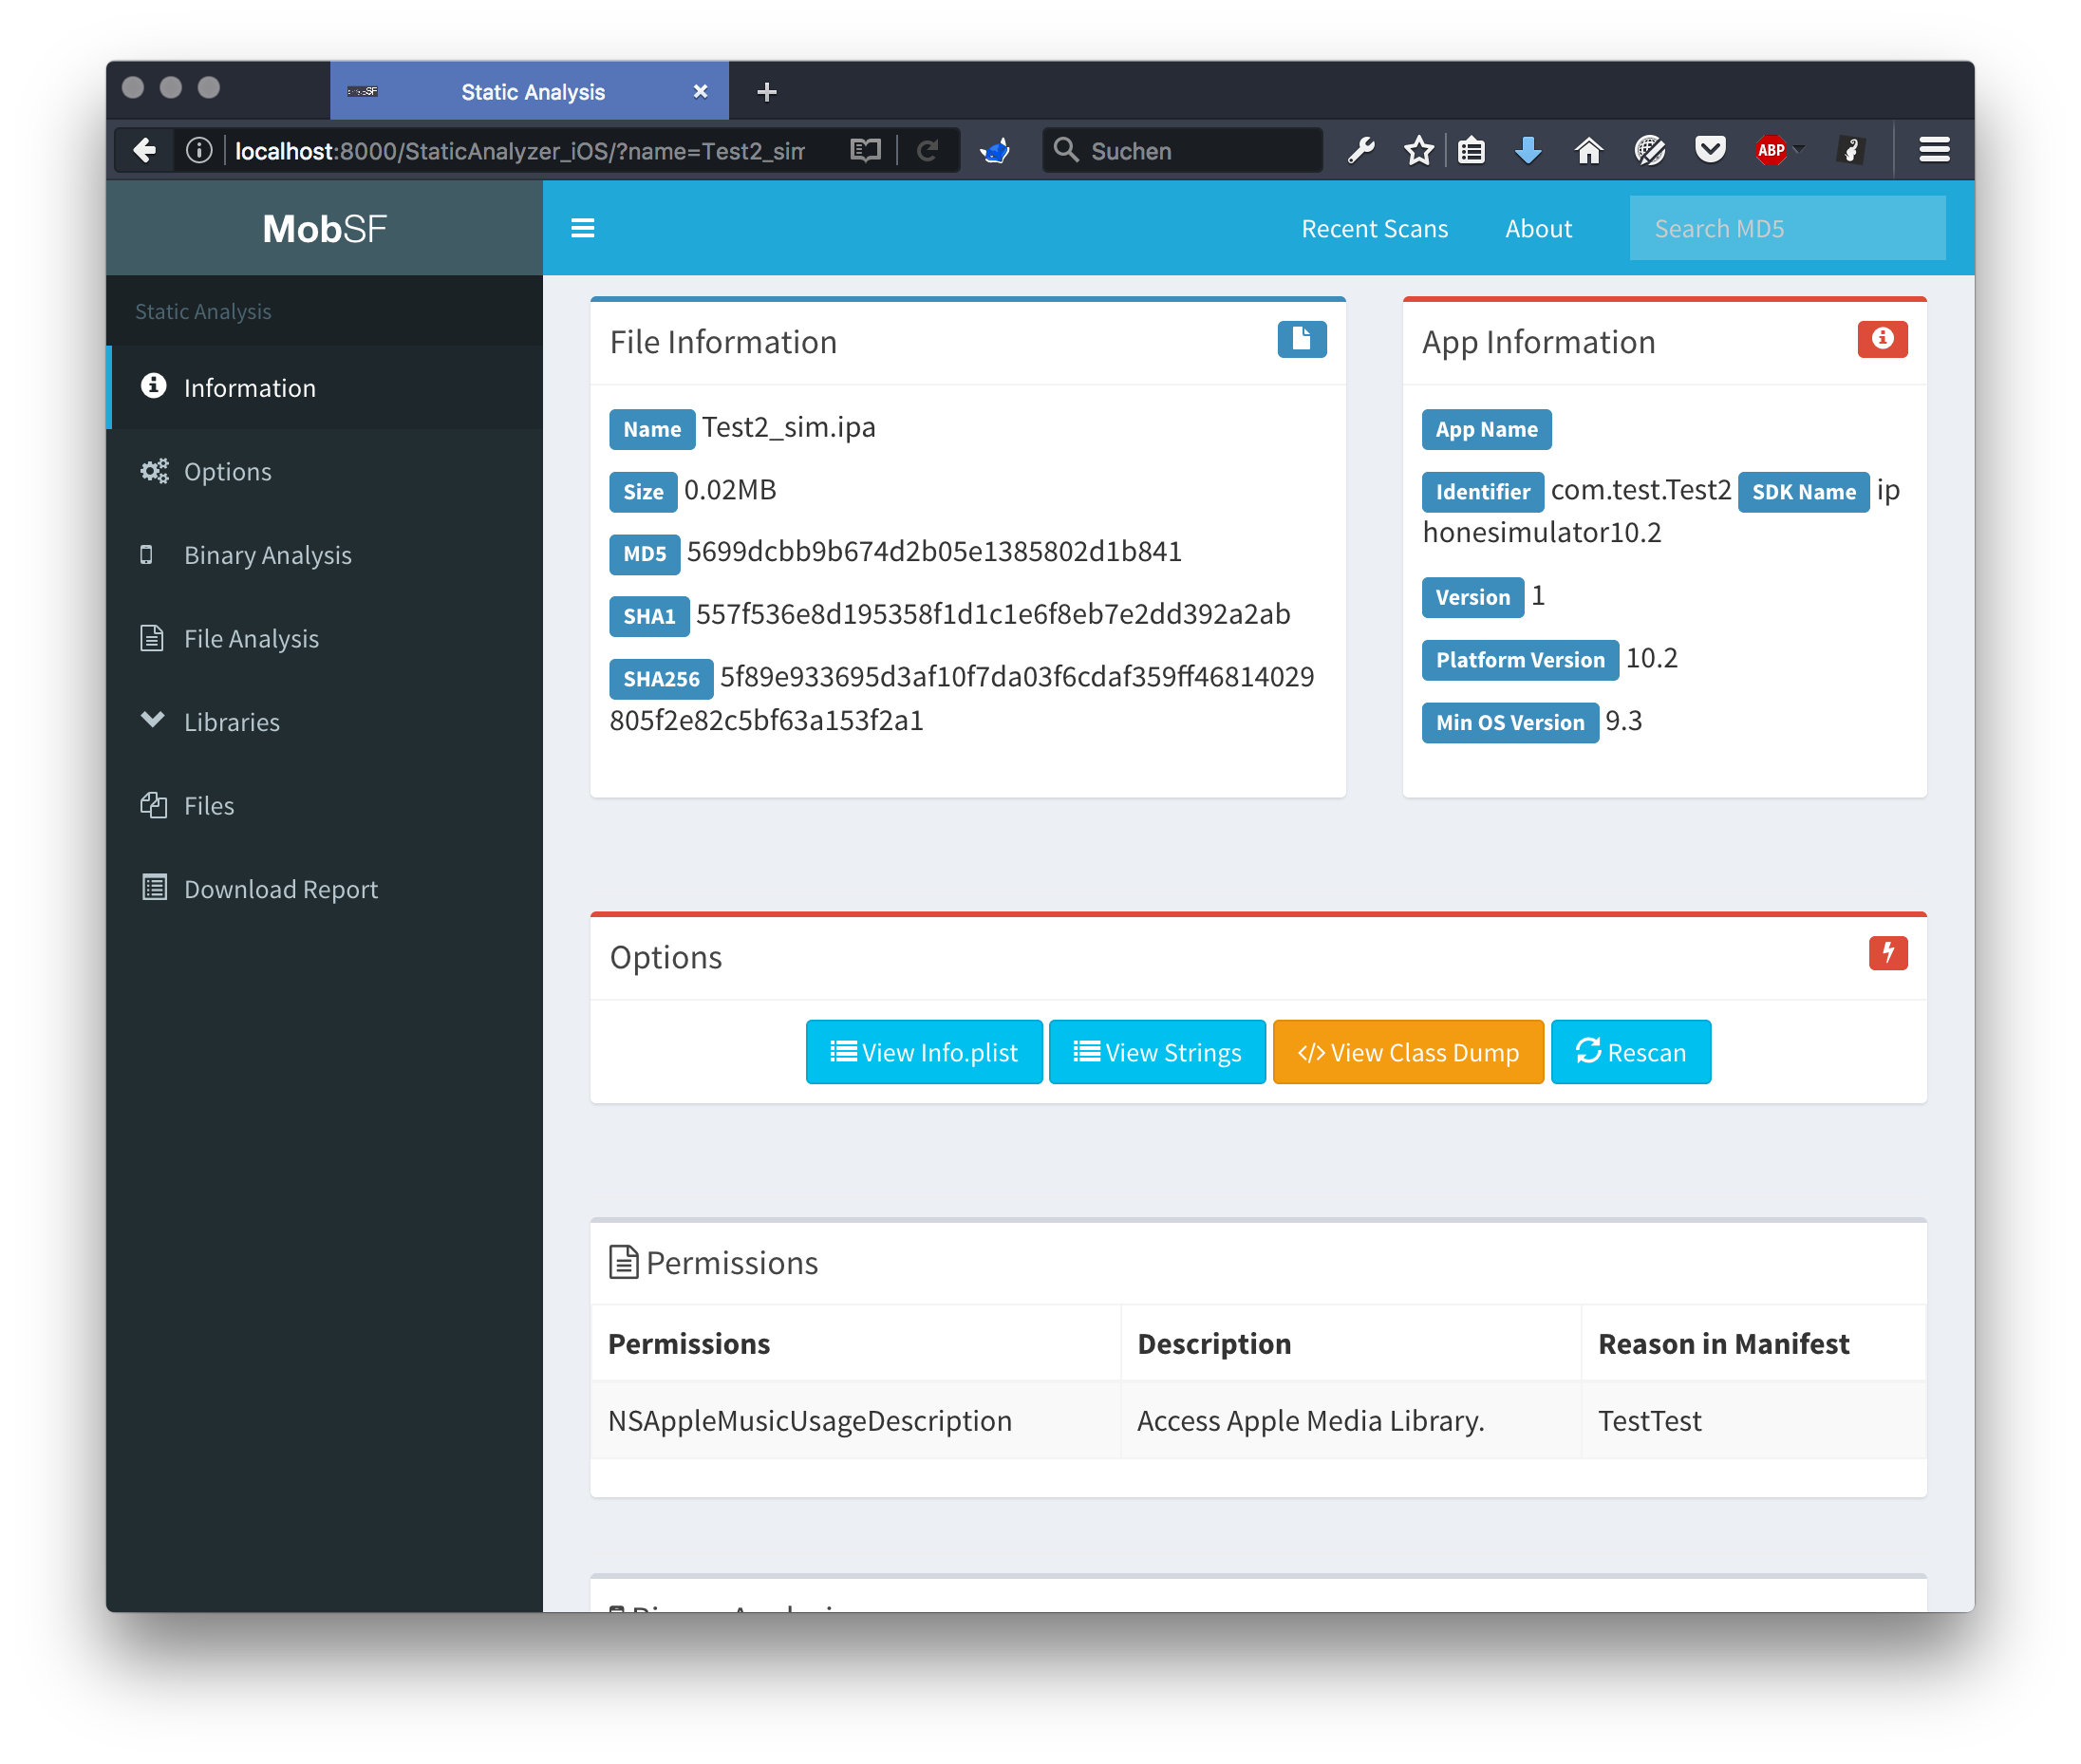
\includegraphics[width=\textwidth]{bilder/pentest_mobile_anwendungen/weiterentw_mobsf/permisson_check.png}
	\caption{Permission-Check-Ergebnis für eine App mit Bluetooth-Berechtigung}
	\label{fig:permission_check}
\end{figure}

\subsubsection{Erkennung von ungesicherten Verbindungen}\label{ref:WeitMobSFErkennungVonUngesichertenVerbindungen}
Wie in \ref{ref:inseccon} unter "`Ungesicherte Verbindungen beschrieben"', müssen ab \textit{iOS} 9.0 Apps den  RFC-Standard 2818\footnote{\url{https://tools.ietf.org/html/rfc2818}} nutzen, um Verbindungen zu Webseiten oder APIs aufzubauen.\\

Daher wurde \textit{MobSF} um ein Feature ergänzt, welches die \textit{Info.plist} auf Ausnahmen überprüft. Der simple Code ist unter Listing \ref{lis:NSAppTransportSecurity} dargestellt.\\

\begin{figure}
	\begin{lstlisting}
def __check_insecure_connections(p_list):
    '''Check info.plist for insecure connection configurations.'''
    print "[INFO] Checking for Insecure Connections"

    insecure_connections = []

    if 'NSAppTransportSecurity' in p_list:
        ns_app_trans_dic = p_list['NSAppTransportSecurity']
        if 'NSExceptionDomains' in ns_app_trans_dic:
            for key in ns_app_trans_dic['NSExceptionDomains']:
                insecure_connections.append(key)

    return insecure_connections
	\end{lstlisting}
	\caption{Auslesen von Ausnahmen bezüglich der TLS-Konfiguration aus der Info.plist}
	\label{lis:NSAppTransportSecurity}
\end{figure}


Werden Ausnahmen gefunden, werden diese in der HTML-Oberfläche dargestellt. Ein Beispiel ist in TODO zu sehen.


\subsubsection{Dynamische Analyse über Simulator}
Im Rahmen dieser Masterarbeit wurden ebenfalls Möglichkeiten getestet, wie eine dynamische Analyse von \textit{iOS}-Apps über den "`Simulator"' abgebildet werden könnten.



Erster Versuch
Gestarted aus xcode, app:
\begin{lstlisting}
NSURL *url = [NSURL URLWithString:@"https://api.ipify.org"];
SData *data = [NSData dataWithContentsOfURL:url];
NSString *ret = [[NSString alloc] initWithData:data encoding:NSUTF8StringEncoding];
\end{lstlisting}
Wireshark output:
\begin{figure}[htbp]
	\centering
	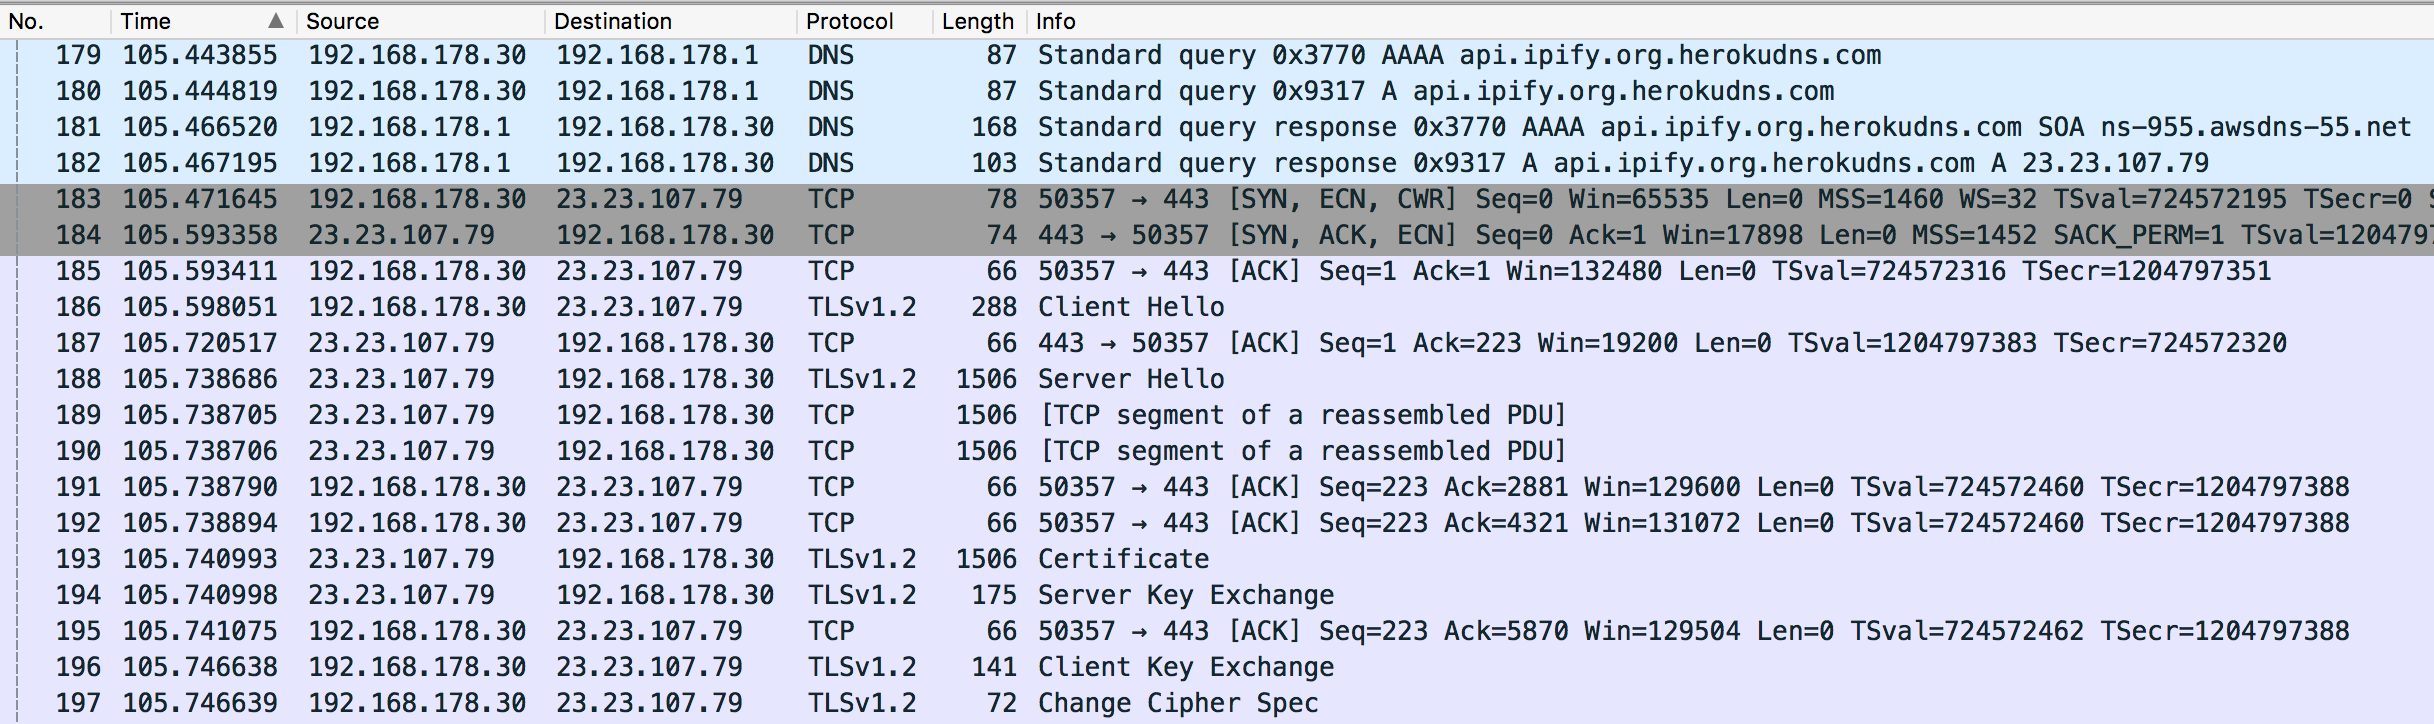
\includegraphics[width=\textwidth]{bilder/pentest_mobile_anwendungen/weiterentw_mobsf/wireshark_simulator.png}
	\caption{Verbindung zu \url{https://api.ipify.org} aus dem iOS-Simulator}
	\label{fig:VergleichLLDBImages}
\end{figure}

Öffnen aus console

mitmproxy vs. http://useyourloaf.com/blog/remote-packet-capture-for-ios-devices/
http://www.binarytides.com/python-packet-sniffer-code-linux/

mitmproxy installieren, Proxy umstellen, https://github.com/ADVTOOLS/ADVTrustStore ausführen und adden, im Iphone aktivieren, neu starten
mitmproxy starten und anfangen zu schreib, lesen und in db speichern
https://github.com/mitmproxy/mitmproxy/blob/0.18.x/examples/flowbasic

LLDB + Code Simulator (siehe weiter oben)

ausführen von aktionen https://developer.apple.com/reference/xctest
xcrun simctl install booted /Users/dominik/Library/Developer/Xcode/DerivedData/Test2-dzkepdcqdrczebclbvysnxcbwrmp/Build/Products/Debug-iphonesimulator/Test2.app
xcrun simctl launch 4A4B2FF5-C435-4ECB-AC49-A4684F133910 Test2

simulator starten einfach über öffnen von App (IPA => Simulator?)

http://www.libimobiledevice.org/
https://github.com/facebook/FBSimulatorControl
http://blog.manbolo.com/2012/04/08/ios-automated-tests-with-uiautomation

http://eightbit.io/post/64319534191/how-to-set-up-an-ios-pen-testing-environment

http://www.testplant.com/dlds/eggplant-mobile-eggon/ ?
http://www.sikuli.org/

remote anzeige
git://git.saurik.com/cydia.git
http://kanaka.github.io/noVNC/ als front interface
http://sharedinstance.net/2013/10/running-tweaks-in-simulator/ vnc server auf Iphone installieren, z.B. https://github.com/niknah/veency

TODO: Öffnen aus Console schreiben
TODO: Netzwerkverkehr mitschneiden schreiben


TODO: Installation VNC-Server auf Simulator testen <-- Kein Chance
TODO: VNC in Web-Oberfläche testen
